\chapter{What is a Proof?}
\begin{pr}\leavevmode
    \begin{enumerate}[label=\textbf{(\alph*)}]
        \item
        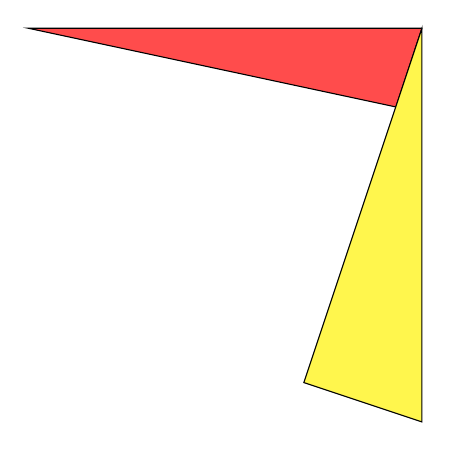
\begin{tikzpicture}
            \draw[fill=red!70] (0,0) -- (5,0) -- (4.67,-1) -- cycle;
            \draw[fill=yellow!70] (5,0) -- (3.5,-4.5) -- (5,-5) --cycle;
        \end{tikzpicture}
        \item item 2
    \end{enumerate}
\end{pr}